% !TeX root=../main.tex
\chapter{پیاده‌سازی}

% ------------ Section 4.1
\section{نوشتن کد قرارداد}
در این بخش به بررسی مراحل و نحوه نوشتن کد قراردادهوشمند پرداخته می‌شود.

% ------------ Sub Section 4.1.1
\subsection{نیازمندی‌های قراردادهوشمند}
نیازمندی‌های اصلی کاپو به ترتیب زیر است.
\begin{itemize}
  \item
هر آدرس در شبکه بتواند یک داده‌ی متنی را به آسان‌ترین و کم هزینه‌ترین روش ممکن به یک توکن NFT تبدیل کند.
  \item
هر آدرس بتواند توکن‌های خود را به اشخاص دیگر انتقال دهد یا در بازارهای معاملات NFT بفروشد.
  \item
در صفحه اول وبسایت تعداد کل توکن‌های ساخته شده تا به حال و تعداد کل دارندگان توکن نمایش داده شود.
  \item
قابلیت‌های قراردادهوشمند تست شده باشد.
\end{itemize}

% ------------ Sub Section 4.1.2
\subsection{ارث‌بری}
با توجه به مزایای ذکر شده در مورد استانداردسازی قراردادهای هوشمند، انتخاب درستی است که برای پیاده‌سازی این کاربری از یکی از استانداردها استفاده شود. ارثبری از استانداردهای یک کتابخانه متن‌باز مزایای زیر را فراهم می‌کند.
\begin{itemize}
  \item
به دلیل وجود کدهای پایه به صورت آماده سرعت توسعه پروژه افزایش می‌یابد.
  \item
ارتباط دیگر پروژه‌ها با پروژه کاپو به راحتی انجام می‌شود.
  \item
امنیت قرارداد و درستی آن حداقل در سطوح پایه‌ای تا حد خوبی تضمین شده است.
\end{itemize}

قراردادهوشمند کاپو از استاندارد ERC721 پیاده‌سازی شده در کتابخانه اپن‌زپلین
\LTRfootnote{
  \url{https://github.com/OpenZeppelin/openzeppelin-contracts}
}
ارث‌بری می‌کند که یکی از معروف ترین کتابخانه‌های پیاده کننده استانداردهای قرارداد هوشمند است.

% ------------ Sub Section 4.1.3
\subsection{توجه به هزینه تراکنش و نوع توابع}
در نوشتن یک قراردادهوشمند باید به نکات زیر توجه کنیم.
\begin{itemize}
  \item
میزان حافظه‌ای که اشغال می‌کنیم.
  \item
حجم بایت‌کد.
  \item
میزان عملیات هر متد، به خصوص متدهایی که مکررا مورد استفاده کاربر قرار می‌گیرند.
  \item
نوع هر متد، که مشخص می‌کند هر متد تا چه حد روی شبکه بلاکچین تغییر ایجاد می‌کند.
\end{itemize}

توجه نکردن به هریک از این موضوعات باعث می‌شود که قراردادهوشمند به اندازه کافی بهینه عمل نکند و کاربر وادار به پرداخت gas fee یا هزینه تراکنش بیشتر شود. یکی از مهمترین نکاتی که برای بهینه‌تر رفتار کردن قراردادهوشمند باید به آن توجه کنیم نوع هر متد است.

اگر متدی از نوع pure تعریف شود به این معنی است که به هیچ اطلاعاتی از شبکه بلاک‌چین نیاز ندارد و همه‌ی اطلاعاتی که لازم دارد را در اسکوپ
\LTRfootnote{Scope}
خودش دارد. اگر متدی از نوع view باشد به این معنی است که به اطلاعاتش روی شبکه بلاکچین نیاز دارد اما فقط می‌خواهد که آن‌ها را بخواند و نمیخواهد تغییری در آن‌ها ایجاد کند. این دو نوع متد نیازی به پرداخت کارمزد تراکنش توسط کاربر ندارند، اما اگر در تعریف متدی ذکر نشود که یکی از این دو نوع است، اینطور در نظر گرفته می‌شود که نیاز به بروزرسانی اطلاعاتش در شبکه بلاکچین دارد و از کاربری که آن را فراخوانی کرده است هزینه تراکنش دریافت می‌شود.


% ------------ Sub Section 4.1.4
\subsection{جزئیات فنی پیاده‌سازی}
مینت کردن در این قرارداد به آدرس‌های مشخص محدود نیست و همه می‌توانند توکن بسازند. بسیاری از قراردادها برای صرفه‌جویی در هزینه تراکنش کاربران اکثر اطلاعات مربوط به توکن‌ها را در قرارداد نگه نمیدارند و فقط داده‌های بسیار مهم توکن را در شبکه بلاکچین نگهداری می کنند. از آنجایی که کاپو یک قرارداد همه منظوره است و ممکن است استفاده‌های فراوانی داشته باشد، تصمیم‌گیری این مورد به عهده کاربر قرارداد گذاشته می‌شود.

در کاپو آیدی هر توکن از hash داده‌های توکن به دست می‌آید. این نحوه عملکرد چند مزیت ایجاد می‌کند. به این ترتیب هیچ دو توکنی نمی‌توانند داده‌های یکسان داشته باشند، زیرا در این صورت آیدی آن‌ها باید یکسان باشد و این امکان پذیر نیست زیرا آیدی توکن‌ها یکتاست. همچنین آیدی توکن‌ها دیگر ترتیبی نخواهند بود و ترتیب ساخت توکن‌ها مشخص نخواهد بود.

در یک قرارداد ERC721 استاندارد فقط آیدی توکن‌ها ذخیره می‌شود. در کاپو علاوه بر آیدی توکن‌ها یک map از آیدی توکن‌ها به داده‌ی آن‌ها با نام tokenDatas نیز نگهداری می‌شود. همچنین در کاپو map دیگری نیز از آدرس به لیست توکن‌های آن آدرس با نام ownerTokens نگهداری می‌شود. متغیر اول کمک می‌کند که با داشتن آیدی یک توکن به راحتی داده‌های آن توکن به دست آورده شوند. متغیر دوم نیز کمک می‌کند که به راحتی بتوان توکن‌های یک آدرس را به دست آورد. دو متغیر دیگر با نام‌های numberOfTokenHolders و numberOfMintedTokens نیز در کاپو نگه‌داشته می‌شوند که برای نمایش آمار استفاده از قرارداد در صفحه اصلی اپلیکیشن مورد استفاده قرار می‌گیرند.

متد mint به نحوی نوشته شده است که برای عموم قابل استفاده باشد. پس از محاسبه hash داده‌ی توکن از آن به عنوان آیدی توکن استفاده می‌کند، توکن را می‌سازد و متغیرهای tokenDatas و numberOfMintedTokens را بروزرسانی می‌کند.

\begin{figure}[ht]
\centerline{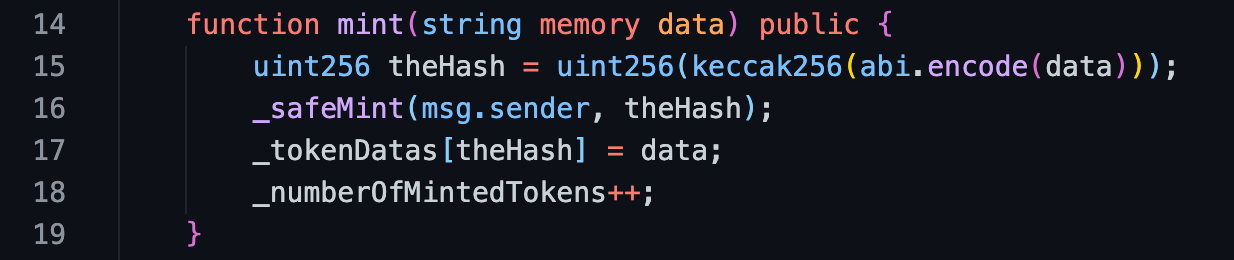
\includegraphics[width=12cm]{mint.png}}
\caption{پیاده‌سازی تابع mint}
\label{fig:mint}
\end{figure}

متد afterTokenTransfer از استاندارد ERC721 به نحوی بازنویسی
\LTRfootnote{Overwrite}
شده است که پس از هر انتقال توکن با بررسی آدرس‌های مبدا و مقصد، متغیر‌های numberOfTokenHolders و numberOfMintedTokens و ownerTokens را بروزرسانی کند.

\begin{figure}[ht]
\centerline{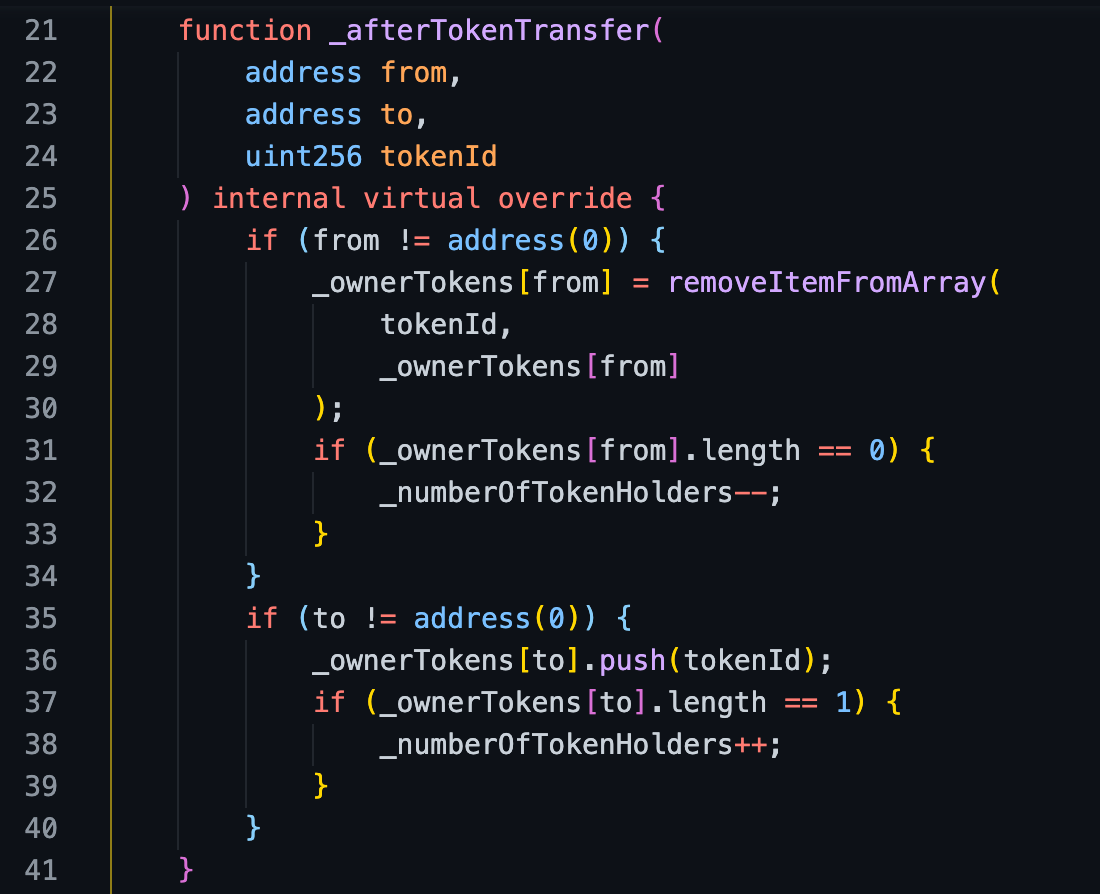
\includegraphics[width=12cm]{afterTokenTransfer.png}}
\caption{پیاده‌سازی تابع afterTokenTransfer}
\label{fig:afterTokenTransfer}
\end{figure}

متد جدیدی با نام getUserTokens نیز نوشته شده است که در استاندارد ERC721 به صورت پیش‌فرض وجود ندارد. این متد با گرفتن یک آدرس و استفاده از ownerTokens و tokenDatas دو خروجی برمی‌گرداند، لیستی از آیدی توکن‌های آدرس و لیستی از داده‌های توکن‌های آدرس.

\begin{figure}[ht]
\centerline{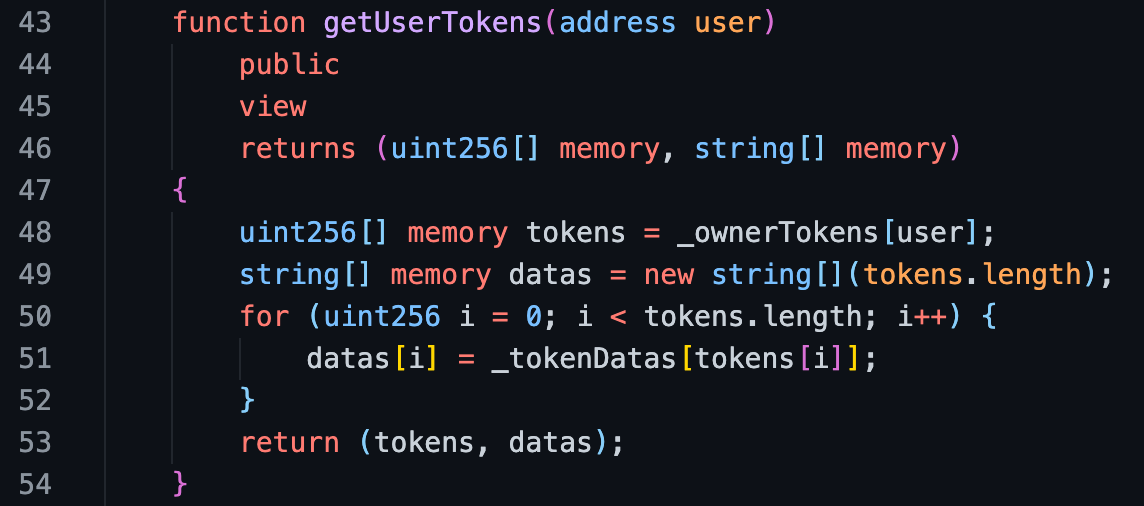
\includegraphics[width=12cm]{getUserTokens.png}}
\caption{پیاده‌سازی تابع getUserTokens}
\label{fig:getUserTokens}
\end{figure}

همچنین از آنجایی که سالیدیتی به طور پیش‌فرض امکان حذف یک داده از یک آرایه با داشتن مقدار آن را ندارد، عدم وجود این قابلیت هزینه‌بر بودن آن است، در سالیدیتی توسعه دهندگان به استفاده از map و دوری از array ها تشویق می‌شوند. اما برای نمایش نحوه ارث‌بری از دو یا چند قرارداد پدر، برای کاپو یک قرارداد به نام Helper نوشته شد که این قابلیت را فراهم می‌کند. کاپو علاوه بر
\lr{ERC721}
از قرارداد Helper نیز ارث‌بری می‌کند.

\begin{figure}[ht]
\centerline{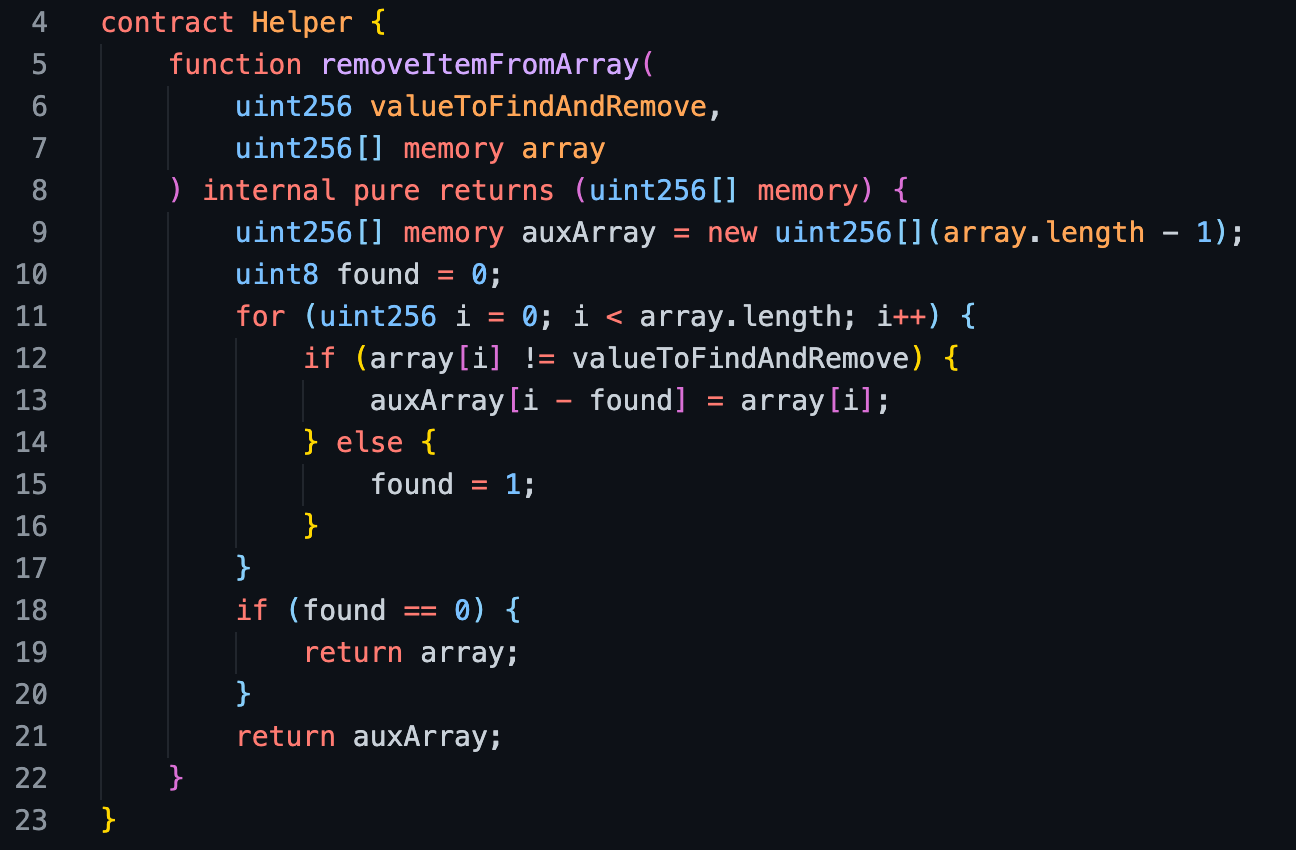
\includegraphics[width=12cm]{Helper.png}}
\caption{پیاده‌سازی قرارداد Helper}
\label{fig:Helper}
\end{figure}

% ------------ Section 4.2
\section{نوشتن و اجرای تست‌ها}
پیش‌تر اشاره شد که از مزیت‌های ارث‌بری از کتابخانه‌های متن‌باز معروف این است که احتمال وجود خطا و مشکل امنیتی به شدت کمتر می‌شود. یکی از دلایل این مسئله این است که این کتابخانه‌ها پوشش تستی به شدت بالایی دارند. به همین دلیل می‌توان تا حدی به عملکرد قرارداد پدر اطمینان خاطر داشت و بیشتر روی تست کردن قابلیت‌های اضافه شده در قراردادهوشمند فرزند تمرکز داشت.

در کاپو برای هر عملکرد قرارداد تست نوشته شده است. یکی از ساده‌ترین تست‌های نوشته شده تست فرآیند ساخت یک توکن است که در آن پس از دیپلوی قرارداد با فراخوانی متد mint یک توکن ساخته می‌شود و سپس با فراخوانی متد balanceOf دارایی آدرس سازنده توکن بررسی می‌شود و انتظار می‌رود که پس از ساخت یک توکن، دارایی آدرس سازنده توکن یک باشد. این تست را می‌توان در تصویر زیر مشاهده کرد.

\begin{figure}[ht]
\centerline{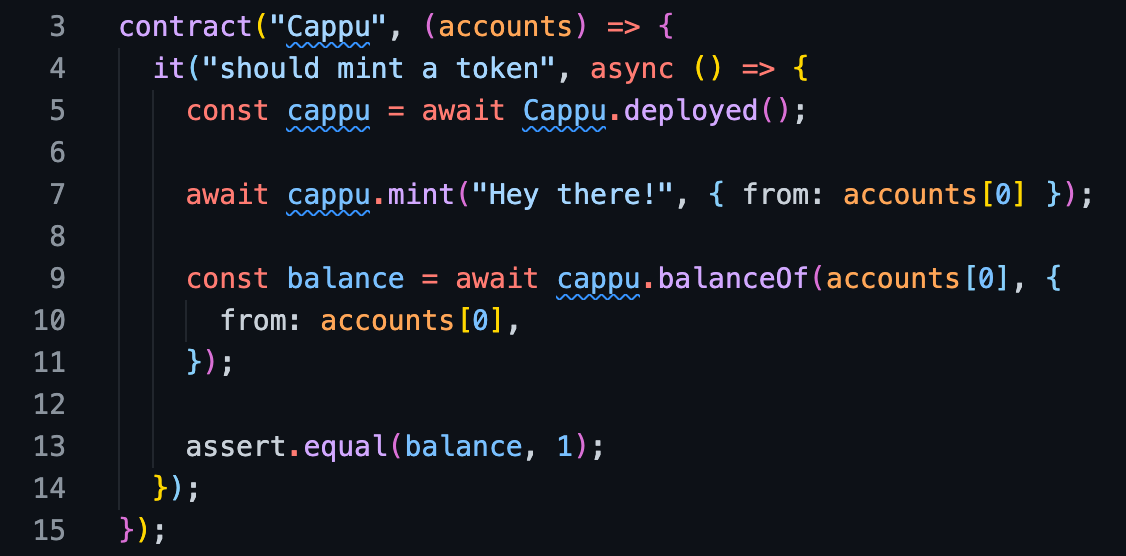
\includegraphics[width=12cm]{mint-test.png}}
\caption{نمونه یکی از تست‌های قرارداد کاپو}
\label{fig:mint-test}
\end{figure}

پس از نوشته شدن تست‌ها می‌توان آن‌ها را با اجرای دستور
\lr{truffle test}
اجرا کرد. این دستور پس از اجرای تست‌ها نتیجه و زمان اجرای هر تست را به عنوان خروجی نمایش می‌دهد. نمونه اجرای این دستور را می‌توان در تصویر زیر مشاهده کرد.

\begin{figure}[ht]
\centerline{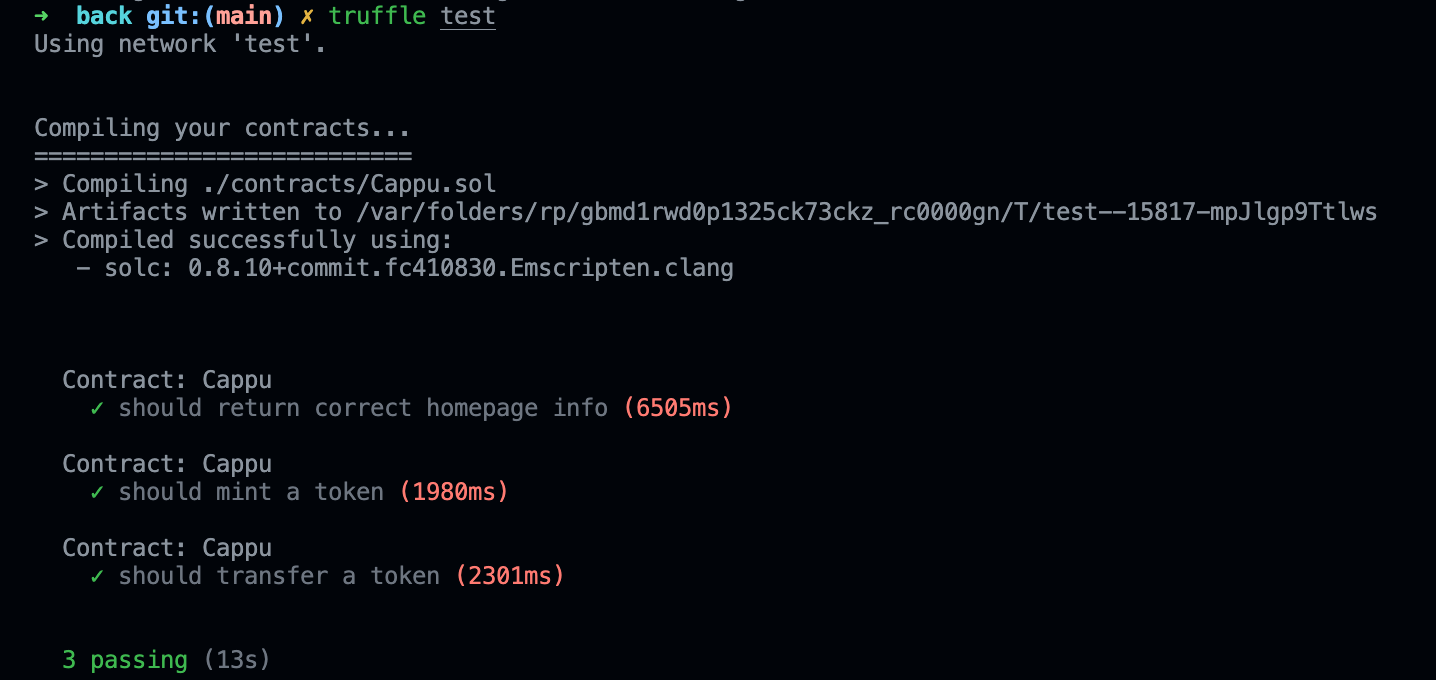
\includegraphics[width=12cm]{test-output.png}}
\caption{نمونه خروجی اجرای تست‌های قرارداد}
\label{fig:test-output}
\end{figure}

% ------------ Section 4.3
\section{دیپلوی قرارداد روی شبکه تستی Ropsten}
تا اینجا قراردادهوشمند نوشته و تست شده است، در این مرحله روی شبکه تستی Ropsten دیپلوی می‌شود. فرآیند دیپلوی شدن کاپو به کمک چارچوب ترافل قدم به قدم شرح داده می‌شود.

\subsection{یافتن آدرس یکی از نود‌های شبکه برای ارسال تراکنش دیپلوی قرارداد به آن}
آدرس نود‌های یک شبکه بلاکچین همه به صورت عمومی در دسترس هستند زیرا نودها باید بتوانند یکدیگر را ببینند. راه‌های زیادی برای به دست آوردن آدرس یک نود وجود دارد. یکی از آسان‌ترین راه‌های به دست آوردن آدرس یکی از نود‌های شبکه مراجعه به وبسایت ماینر است. برای این پروژه از وبسایت Moralis
\LTRfootnote{
  \url{https://moralis.io}
}
برای پیدا کردن آدرس نود شبکه استفاده شد.

\begin{figure}[ht]
\centerline{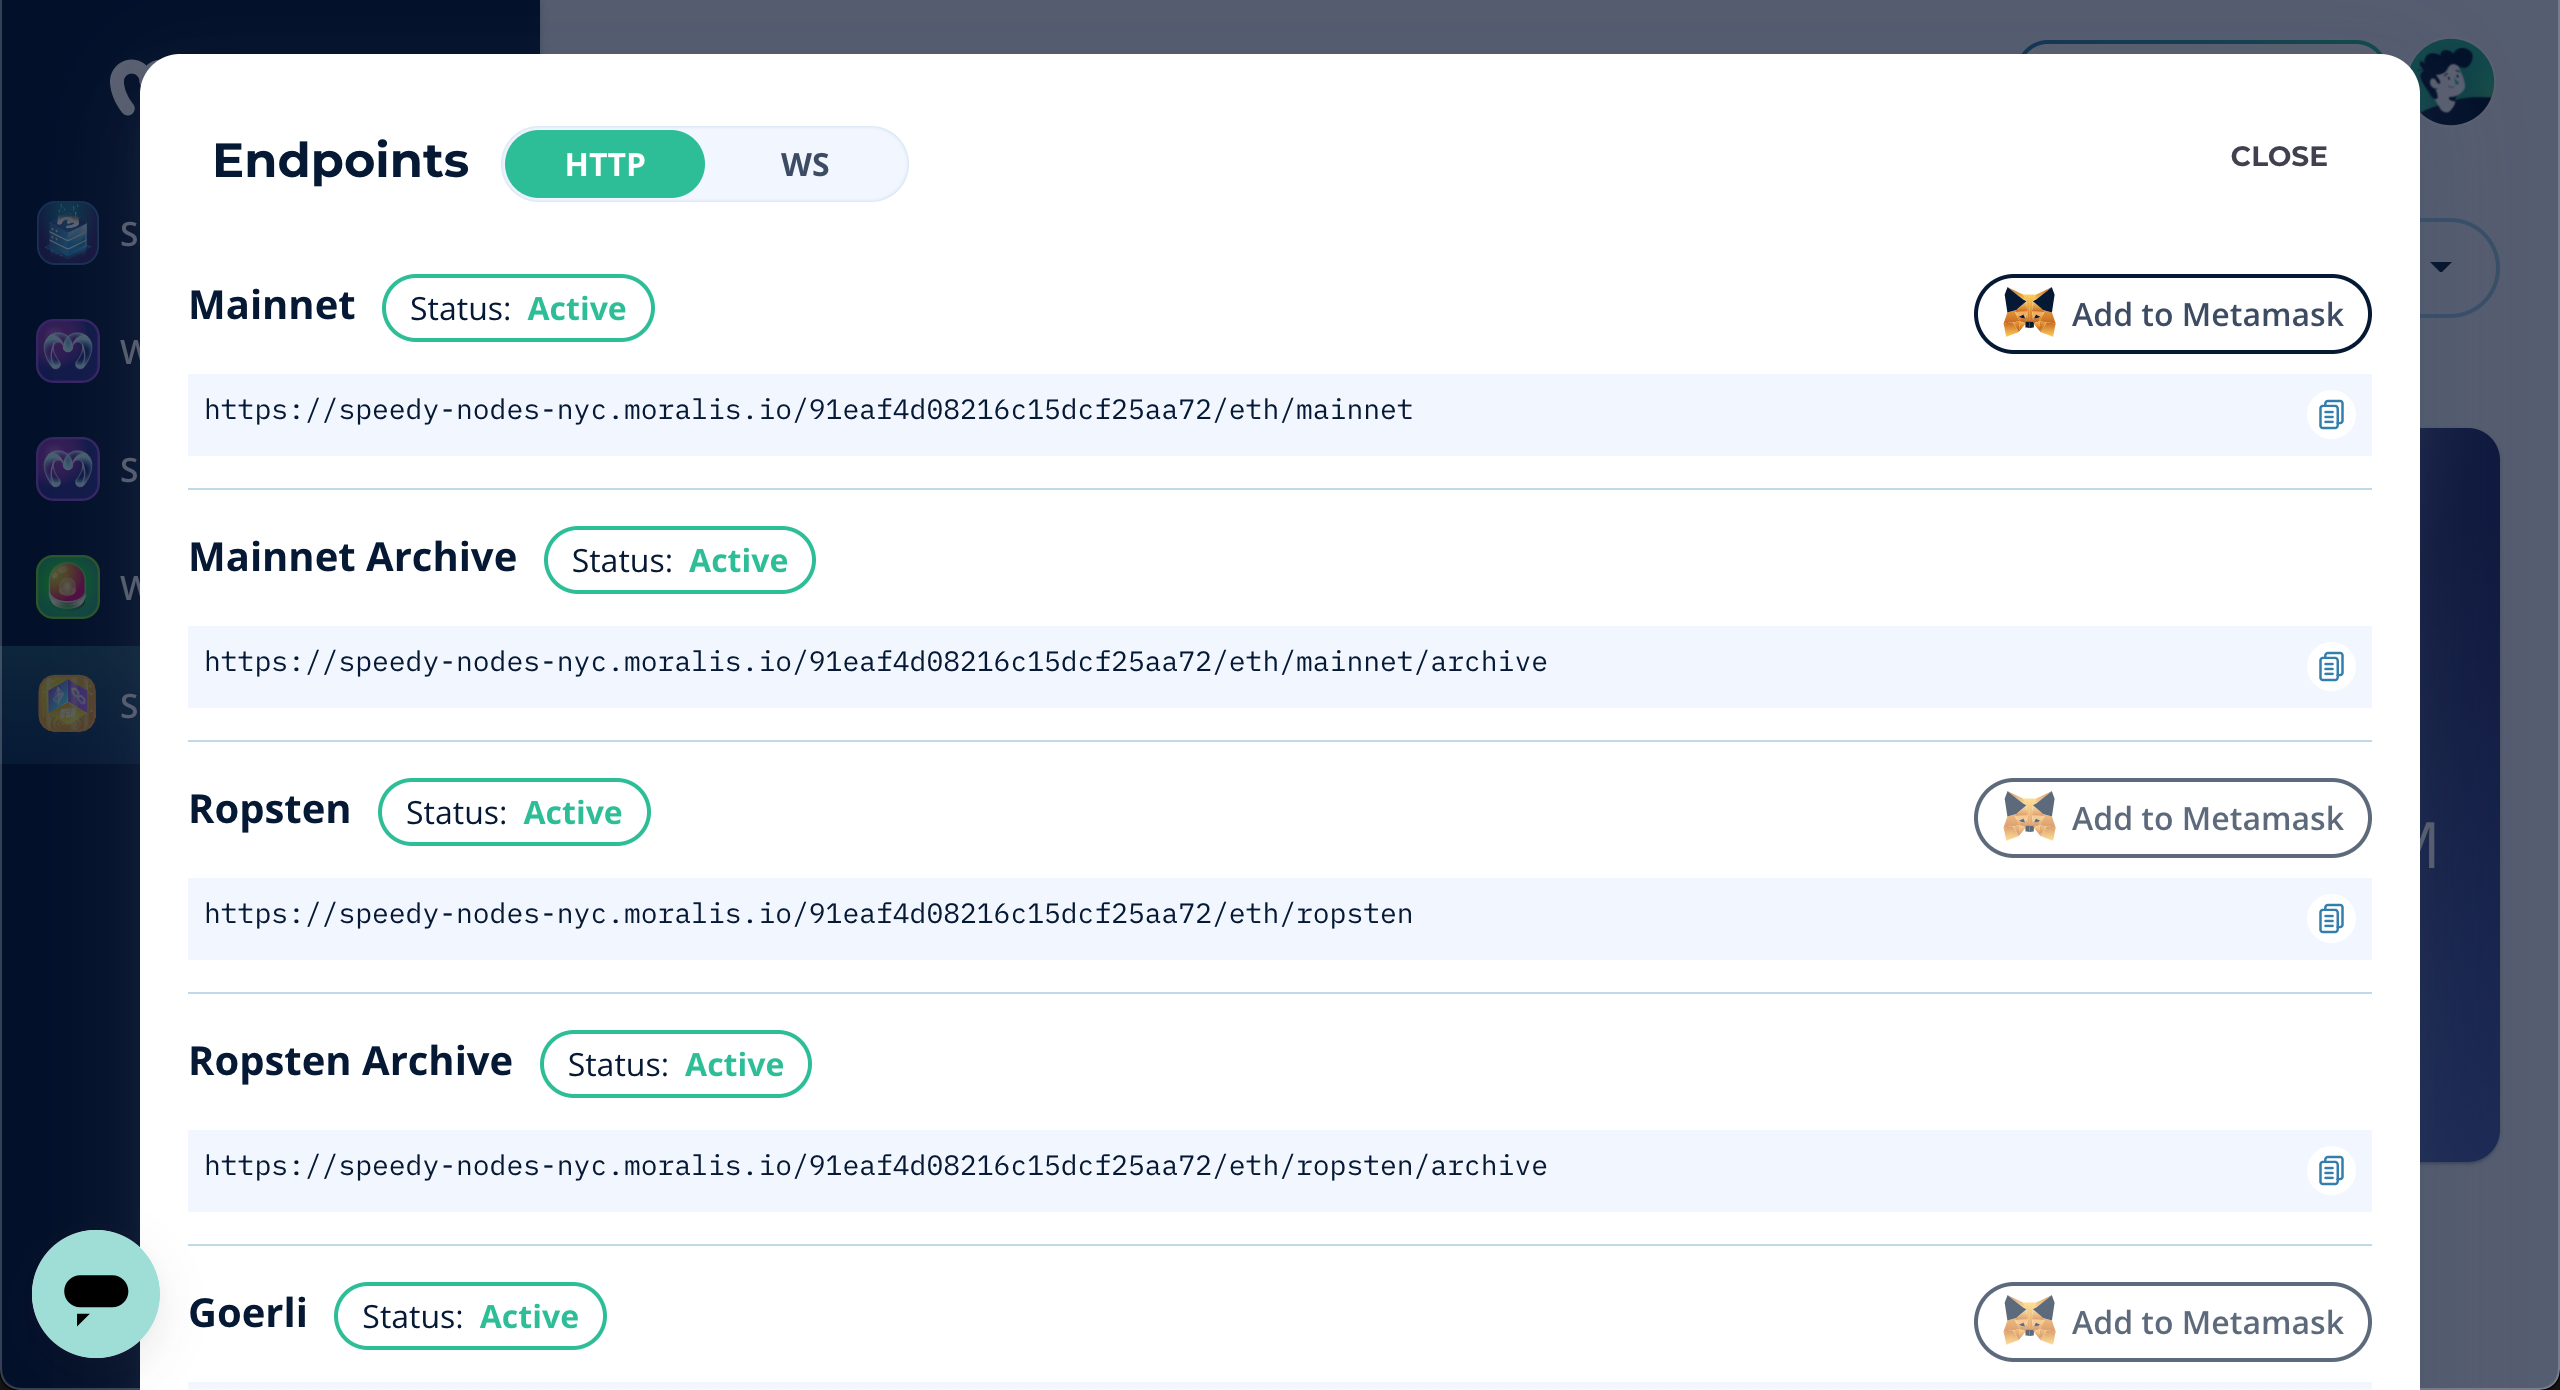
\includegraphics[width=12cm]{moralis.png}}
\caption{دریافت آدرس یکی از نود‌های شبکه از وبسایت Moralis}
\label{fig:moralis}
\end{figure}

\subsection{اضافه شدن اطلاعات شبکه مورد نظر به تنظیمات ترافل}
هنگامی که به کمک دستور
\lr{truffle init}
یک پروژه ترافل ساخته می‌شود، فایلی با نام truffle-config.js ساخته می‌شود. تنظیمات مربوط به ترافل در این فایل نوشته شده‌است. برای این که ترافل شبکه مورد نظر را بشناسد باید اطلاعات آن شبکه در این فایل نوشته و شبکه‌ی جدیدی تعریف شود. برای تعریف شبکه از آدرسی که در گام قبل به دست آمد استفاده می‌شود و مانند تصویر زیر شبکه‌ی جدیدی تعریف می‌شود.

\begin{figure}[ht]
\centerline{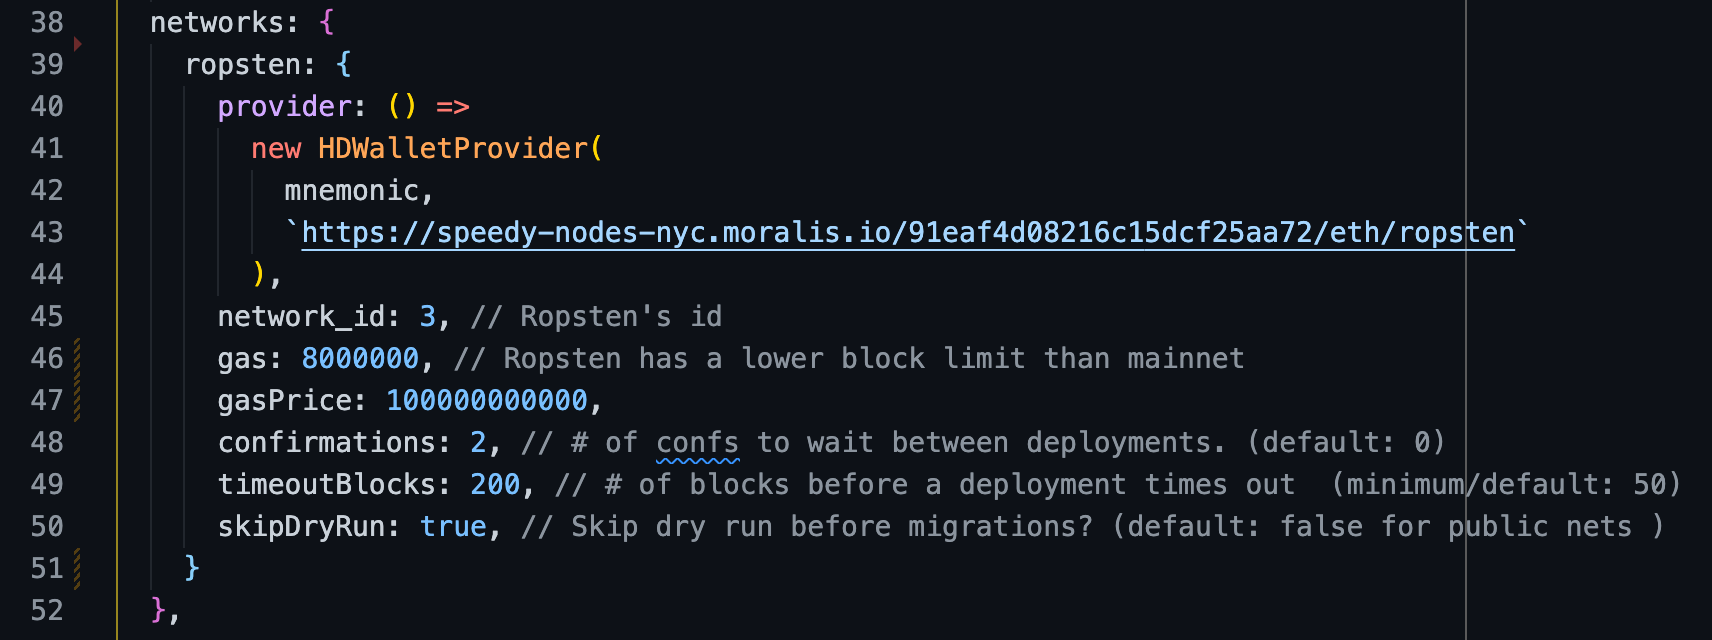
\includegraphics[width=12cm]{network-config.png}}
\caption{اضافه کردن شبکه Ropsten به شبکه‌های ترافل}
\label{fig:network-config}
\end{figure}


\subsection{آماده شدن mnemonics}
برای انجام این پروژه به کمک دستور
\lr{npm mnemonics}
یک آدرس تستی ساخته می‌شود. این دستور، mnemonics متناسب با این آدرس را به عنوان خروجی می‌دهد. دقت کنید که برای دیپلوی روی
\gls{Mainnet}
حتما باید از mnemonics مربوط به یک کیف پول واقعی استفاده شود و اطلاعات ان در اختیار کسی قرار نگیرد.

\begin{figure}[ht]
\centerline{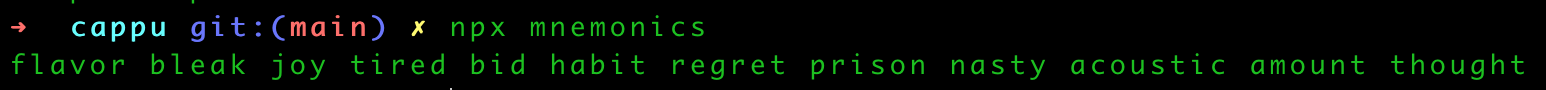
\includegraphics[width=12cm]{mnemonics.png}}
\caption{ایجاد mnemonics تستی}
\label{fig:mnemonics}
\end{figure}


\subsection{استفاده از کیف پول ایجاد شده در تنظیمات ترافل}
ترافل برای این که بتواند از کیف‌پول برای انجام تراکنش‌ها استفاده کند باید به mnemonics یا کلید خصوصی آن دسترسی داشته باشد. به این منظور فایلی با نام secrets.json در دایرکتوری اصلی برنامه ساخته می‌شود و mnemonics کیف پول به شکل زیر در آن قرار داده می‌شود.

\begin{figure}[ht]
\centerline{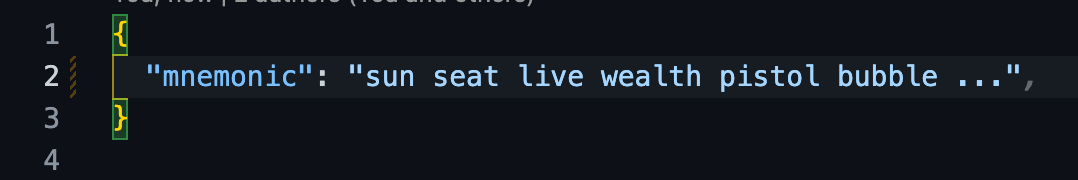
\includegraphics[width=12cm]{mnemonics-in-secrets.png}}
\caption{قراردادن mnemonics در فایل secrets.json}
\label{fig:mnemonics-in-secrets}
\end{figure}

سپس در تنظیمات ترافل باید ذکر شود که می‌تواند آدرس کیف‌پول را در این آدرس پیدا کند.

\begin{figure}[ht]
\centerline{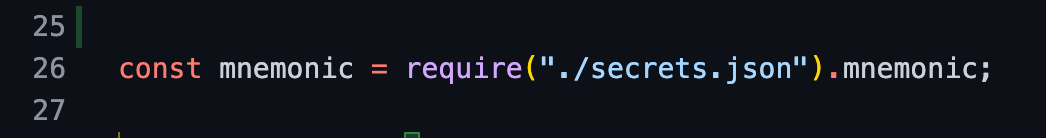
\includegraphics[width=12cm]{secrets-in-config.png}}
\caption{معرفی فایل secrets.json در تنظیمات ترافل}
\label{fig:secrets-in-config}
\end{figure}


\subsection{نصب کیف‌پول hdwallet}
ترافل برای استفاده از mnemonics کیف پول ما نیاز به نصب پکیج hdwallet-provider دارد، این پکیج کاربری‌های یک کیف پول دیجیتال از جمله امضا و ارسال تراکنش بر روی شبکه بلاکچین را در اختیار ترافل قرار می‌دهد. این پکیج با اجرای دستور
\lr{npm install –save-dev @truffle/hdwallet-provider}
نصب می‌شود.  پس از نصب کیف پول در تنظیمات ترافل در فایل truffle-config.js ذکر می‌شود که از این کیف‌پول استفاده شود.

\begin{figure}[ht]
\centerline{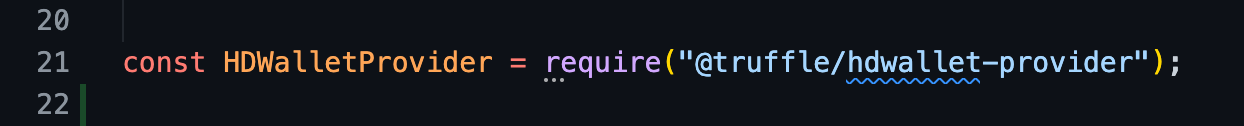
\includegraphics[width=12cm]{wallet-in-config.png}}
\caption{استفاده از کیف‌پول hdwallet در تنظیمات ترافل}
\label{fig:wallet-in-config}
\end{figure}


\subsection{انتخاب شبکه اضافه شده}
حال هنگام ورود به خط فرمان ترافل مانند تصویر زیر شبکه مورد نظر انتخاب می‌شود.

\begin{figure}[ht]
\centerline{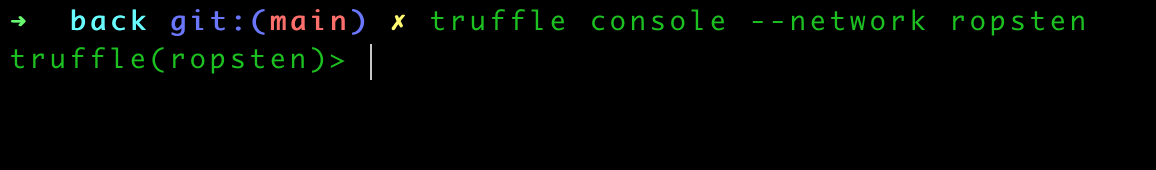
\includegraphics[width=12cm]{truffle-console.png}}
\caption{ورود به خط فرمان ترافل با انتخاب شبکه Ropsten}
\label{fig:truffle-console}
\end{figure}


\subsection{بررسی آدرس کیف‌پول و موجودی آن}
برای دیپلوی یک قرارداد هوشمند باید آدرس دیپلوی کننده آن بتواند هزینه تراکنش دیپلوی را پرداخت کند. در صورتی که دیپلوی بر روی یک شبکه تستی انجام می‌شود باید با استفاده از یک faucet روی شبکه تستی به میزان کافی پول تستی دریافت شود.

برای دریافت آدرس‌های کیف‌پول از دستور زیر در خط فرمان ترافل استفاده می شود.

\begin{figure}[ht]
\centerline{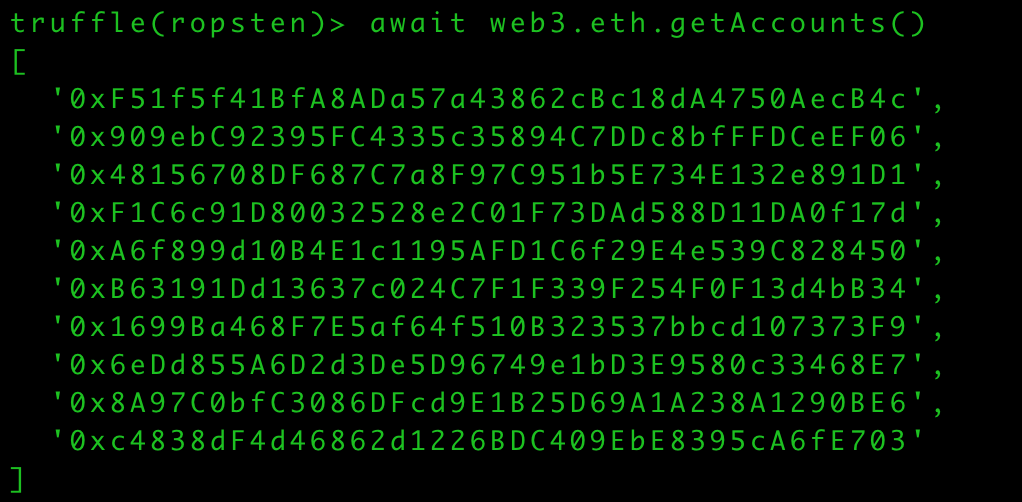
\includegraphics[width=12cm]{get-addresses.png}}
\caption{دریافت آدرس‌های کیف‌پول در خط فرمان ترافل}
\label{fig:get-addresses}
\end{figure}

برای دریافت مانده حساب آدرس، دستور زیر در خط فرمان ترافل اجرا می‌شود.

\begin{figure}[ht]
\centerline{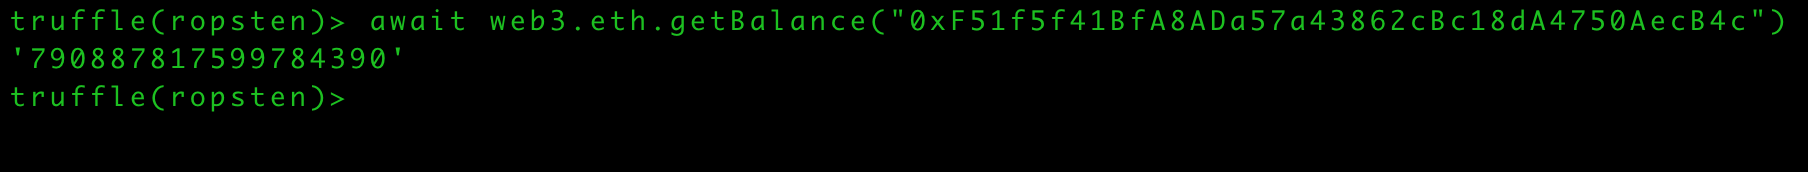
\includegraphics[width=12cm]{get-wallet-balance.png}}
\caption{دریافت موجودی کیف‌پول در خط فرمان ترافل}
\label{fig:get-wallet-balance}
\end{figure}


\subsection{دیپلوی قراردادهوشمند روی شبکه بلاکچین}
پس از اطمینان از توانایی پرداخت کارمزد تراکنش با استفاده از دستور migrate در خط فرمان ترافل قراردادهوشمند روی شبکه بلاکچین دیپلوی می‌شود.


\subsection{اطمینان از صحت دیپلوی قراردادهوشمند}
س از اتمام دیپلوی قرارداد هوشمند برای اطمینان از به درستی انجام شدن فرآیند دیپلوی قرارداد، می‌توان از
\glspl{Block Explorer}
بلاکچین استفاده کرد. برای مثال قرارداد هوشمند کاپو بر روی شبکه Ropsten دیپلوی شده است، که با رفتن به وبسایت اتراسکن
\LTRfootnote{
\url{https://etherscan.io}
}
و قراردادن آن روی شبکه Ropsten می‌توان قرارداد دیپلوی شده و تراکنش‌های آن را مشاهده کرد.


\begin{figure}[ht]
\centerline{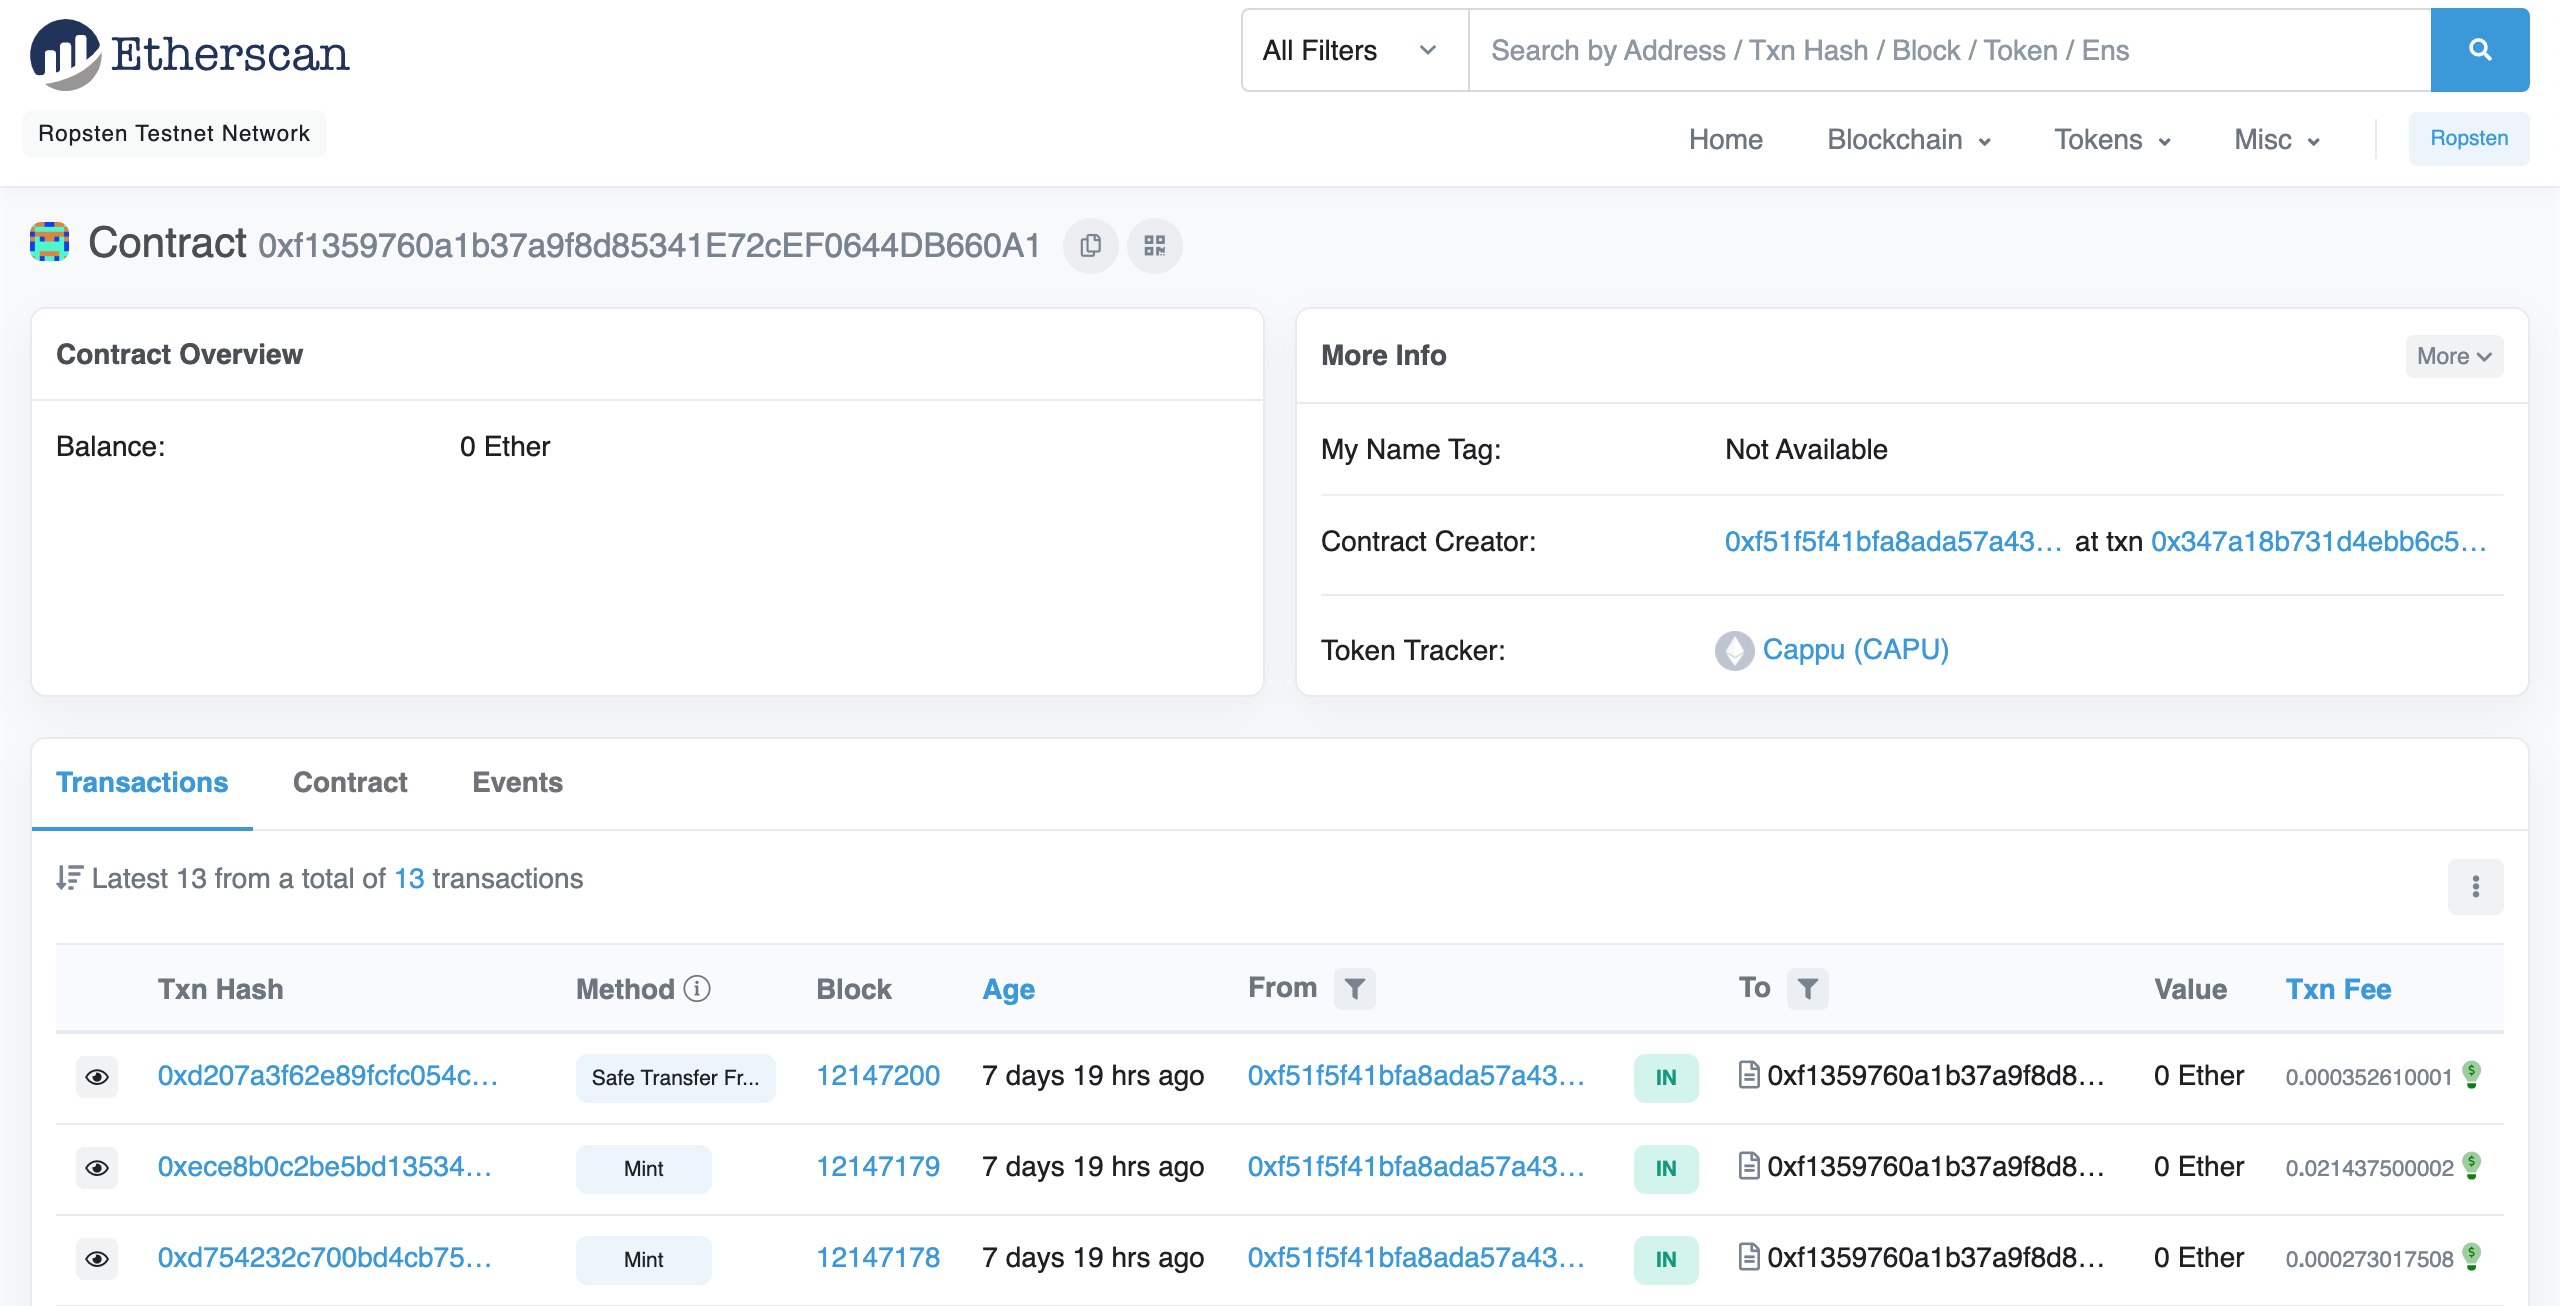
\includegraphics[width=12cm]{etherscan.png}}
\caption{مشاهده قراداد کاپو در Etherscan روی شبکه Ropsten}
\label{fig:etherscan}
\end{figure}


% ------------ Section 4.4
\section{توسعه فرانت، اتصال به قراردادهوشمند و فرآیند دیپلوی}
برای توسعه فرانت‌اند اپلیکیشن، React به عنوان چارچوب مورد استفاده انتخاب شد. ترکیب این چارچوب با استفاده از کتابخانه material-ui که کمک می‌کند در زمان کوتاه بتوان ظاهری زیبا و یکدست در اپلیکیشن ایجاد کرد و کتابخانه
\lr{Web3JS}
که فرانت‌اند را به کیف پول کاربر و شبکه بلاکچین متصل می‌کند، همه‌ی قابلیت‌های مورد نیاز برای توسعه یک فرانت‌اند زیبا و کارآمد را در اختیار توسعه دهنده قرار می‌دهد.

در پوشه اصلی فرانت‌اند فایلی با عنوان config.js وجود دارد. در این فایل علاوه بر ABI قراردادهوشمند سایر اطلاعات مورد نیاز مانند آدرس شبکه، آدرس قرارداد در شبکه و نام شبکه مورد نظر نیز ذخیره می‌شود. هنگام توسعه باید دقت شود که این فایل به قرارداد روی شبکه لوکال متصل شود.

برای استفاده از
\lr{Web3JS}
و اتصال به کیف‌پول کاربر یک فایل به نام connect.js ساخته شد، تمامی اعمال ارتباطی با کیف پول کاربر به عنوان چند تابع در این فایل جمع آوری شده‌اند، این فایل به صورت یک آداپتور میان
\lr{Web3JS}
و کد کاپو عمل می‌کند. تمامی قابلیت‌های مورد نیاز مانند اتصال به کیف‌پول و
\gls{Login}
کاربر،
\gls{Logout}
کاربر، گرفتن آدرس و شبکه‌ی کیف پول و ... در این فایل انجام می‌شود.

فرانت‌اند کاپو پس از تایید کاربر و دریافت آدرس کیف‌پول او، آن را در sessionStorage ذخیره می‌کند، از این طریق متوجه می شود که آیا کاربر وارد شده است یا خیر و با چه آدرسی. کاپو پیش از اتصال به کیف پول کاربر چک می‌کند که کیف پول روی شبکه یکسانی با شبکه فعلی کاپو باشد و در غیر این صورت به کاربر هشدار می‌دهد. همچنین در فرانت‌اند کاپو برای داشتن تجربه کاربری بهتر تلاش شده است. نکاتی مانند عدم نمایش قابلیت‌هایی مانند ساخت و ارسال توکن هنگامی که کیف پول کاربر به اپلیکیشن متصل نیست، جابه‌جایی آسان میان صفحات به کمک react-router، طراحی responsive برای رایانه و گوشی موبایل، نمایش alert ها و error های مناسب به کاربر، نمایش loading هنگامی که تراکنش‌ها در حالت pending هستند و نمایش پیام‌های مناسب با توجه به نتیجه تراکنش‌های کاربر.

برای این که کاربرها بتوانند با قراردادهوشمند ارتباط برقرار کنند نیاز است که فرانت‌اند اپلیکیشن در سروری بارگذاری شود. خوشبختانه گیت‌هاب قابلیت به نام
\lr{Github Pages}
در اختیار کاربرانش قرار می‌دهد که به کمک آن می‌توان فرانت‌اند اپلیکیشن را در آدرسی متناسب با آدرس مخزن کد در گیت‌هاب بارگذاری کرد و کاربران با رجوع به آن آدرس می‌توانند فرانت‌اند اپلیکیشن را ببینند و از آن استفاده کنند.

این قابلیت گیت‌هاب در واقع به این صورت عمل می‌کند که یک برنچ به نام gh-pages در repository پروژه می‌سازد و هربار که دستور دیپلوی پروژه توسط گیت‌هاب اجرا می‌شود، یک بیلد از پروژه می‌گیرد و فایل‌های خروجی بیلد روی این برنچ پوش می‌شوند. سپس این فایل‌ها روی آدرسی متناسب با آدرس repository دیپلوی می‌شوند. برای مثال آدرس ریپازیتوری و فرانت‌اند اپلیکیشن کاپو به صورت زیر است:
\begin{itemize}
  \item
  آدرس ریپازیتوری: \url{https://github.com/bshramin/cappu}
  \item
  آدرس فرانت‌اند: \url{https://bshramin.github.io/cappu}
\end{itemize}
البته دیپلوی شدن فرانت‌اند روی
\lr{Github Pages}
با ایجاد مشکلاتی در routing همراه بود که رفع شدند.


% ------------ Section 4.5
\section{داکرایز شدن، پایپلاین‌ها وگیت}
اقدامات زیر به منظور سرعت بخشیدن و تسهیل فرآیندهای توسعه و دیپلوی انجام شدند.

\subsection{داکرایز شدن تست‌های قراردادهوشمند}
برای سرعت بخشیدن به توسعه قراردادهوشمند، این نیازمندی به وجود آمد که بعد از پوش شدن هر تغییر روی گیت‌هاب تست‌های قرارداد به صورت خودکار اجرا شوند. به این منظور پیش از هر چیز تست‌های قراردادهوشمند باید بتوانند به صورت داکرایز اجرا شوند.

برای داکرایز کردن اجرای تست‌های قرارداد هوشمند، اول سعی در این بود که یک ایمیج داکر پایه که ترافل روی آن نصب شده باشد پیدا شود، اما نسخه ترافل نمونه‌هایی که یافت شد با نسخه مورد نظر همخوانی نداشت. در نتیجه یک ایمیج پایه داکر نوشته شد که داکرفایل آن را می‌توان در گیت‌هاب
\LTRfootnote{
  \url{https://github.com/bshramin/truffle-docker}
}
مشاهده کرد، همچنین این ایمیج داکر در داکرهاب
\LTRfootnote{
  \url{https://hub.docker.com/r/aminbshr/truffle}
}
نیز پوش شد.

سپس داکرفایل دیگری نوشته شد که با استفاده از این ایمیج پایه تست‌های قرارداد را اجرا کند. تست‌های قرارداد در این ایمیج که ترافل بر روی آن نصب شده است با اجرای دستور
\lr{truffle test}
اجرا می‌شود.


\subsection{اجرای خودکار تست‌های قرارداد}
با داشتن داکرفایلی که با بیلد و اجرای آن تست‌های قراردادهوشمند اجرا می‌شوند، تست‌های قراردادهوشمند می‌توانند به عنوان یکی از مراحل پایپلاین پروژه در گیت‌هاب نیز اجرا گردند. به این صورت در هر مرج ریکوئست به برنچ master و با پوش شدن یک کامیت در برنچ master تست‌ها به صورت خودکار در پایپلاین گیت‌هاب اجرا می‌شوند. به این ترتیب سرعت توسعه و اطمینان از کدهای قرارداد بیشتر می‌شود.


\subsection{دیپلوی خودکار فرانت‌اند}
برای ساده‌سازی بیشتر فرآیند دیپلوی فرانت‌اند و سرعت بخشیدن به توسعه آن، این قابلیت پیاده سازی می‌شود که پس از هربار ایجاد تغییر در فرانت‌اند، به جای این که توسعه‌دهنده با اجرای دستوراتی فرانت‌اند را به کمک
\gls{Github Pages}
دیپلوی کند، فرانت‌اند پس از پوش شدن تغییرات جدید روی برنچ اصلی ریپازیتوری دیپلوی می‌شود.

برای پیاده‌سازی این قابلیت از
\lr{Github Actions}
که در واقع پایپلاین‌های گیت‌هاب برای یک پروژه هستند استفاده می‌شود. تنها نکته‌ای که باید به آن توجه شود این است که این استیج از پایپلاین یک تفاوت اصلی با استیج‌های دیگر دارد. استیج‌های دیگر فقط می‌خواهند که کدهای ریپازیتوری را بخوانند و نمی‌خواهند چیزی را در ریپازیتوری تغییر دهند، اما این استیج می‌خواهد که کد‌های فرانت‌اند را بیلد کند و سپس فایل‌های بیلد شده را روی برنچ دیگری به نام gh-pages پوش کند. پس این استیج پایپلاین نیاز به دسترسی پوش کردن کد روی ریپازیتوری دارد.

برای پیاده‌سازی این قابلیت به این صورت عمل می‌شود که نخست یک داکرفایل نوشته می‌شود که در آن کدهای فرانت‌اند بیلد و سپس به کمک
\gls{Github Pages}
روی برنچ gh-pages پوش و دیپلوی می‌شوند. اما این کانتینر برای این که بتواند کدها را روی ریپازیتوری پوش کند نیاز به یک توکن از گیت‌هاب دارد، به همین دلیل برای این داکرفایل یک ENV تعریف می‌شود و هنگامی که در استیج دیپلوی فرانت‌اند این داکرفایل بیلد و اجرا می‌شود توکنی که از گیت‌هاب گرفته شده است به عنوان env به این کانتینر داده می‌شود. به این ترتیب این توکن درون کانتینر داکر وجود خواهد داشت و
\lr{Github Pages}
از آن استفاده خواهد کرد.

